\problemname{Dansgólf}

\illustration{0.4}{dansgolf}{Dæmi um dansgólf}

Hefur þú ekki séð nýja dansgólfið á dansstaðnum Vestur? Það er það heitasta í
bænum um þessar mundir, og unglingarnir bíða í löngum röðum eftir að komast á
gólfið til að dansa!

En þrátt fyrir mikla aðsókn undanfarið hefur reksturinn hjá Vestur ekki gengið
vel, og þeir leita því að öllum mögulegum leiðum til að spara peninga. Til
dæmis er nokkuð dýrt að lýsa upp dansgólfið, svo nú spá þau hvort hægt sé að
slökkva á eitthvað af ljósunum. Auðvitað þarf þó að vera lýsing á öllum þeim
stöðum sem fólk er að dansa á.

Dansgólfið lítur út eins og sýnt er á myndinni hér til hægri. Það samanstendur
af $N$ röðum og $M$ dálkum. Hvert ljós lýsir upp heila skálínu á dansgólfinu,
og hefur hvert ljós sinn eigin lit.

Vestur hefur nú beðið þig um hjálp. Þau gefa þér lista af öllum þeim reitum á
dansgólfinu sem innihalda dansandi fólk, og biðja þig að finna út hver er
fæsti fjöldi ljósa sem þau þurfa að hafa kveikt á þannig að það sé lýsing hjá
öllum þeim sem eru að dansa.

\section*{Inntak}
Fyrsta lína inniheldur þrjár heiltölur $N, M, K$, þar sem $N$ táknar fjölda
raða, $M$ táknar fjölda dálka, og $K$ táknar fjölda reita þar sem fólk dansar.
Síðan fylgja $K$ línur, þar sem hver lína inniheldur tvær heiltölur $x, y$, $1
\leq x \leq N$ og $1 \leq y \leq m$, sem táknar að það sé fólk dansandi á reit
$(x,y)$. Enginn reitur verður gefinn upp oftar en einu sinni.

\section*{Úttak}
Skrifaðu út minnsta fjölda ljósa sem þarf að hafa kveikt á svo að allir reitir
sem hafa dansara séu lýstir.

\section*{Útskýring á sýnidæmi 1}
\begin{figure}[h]
    \centering
    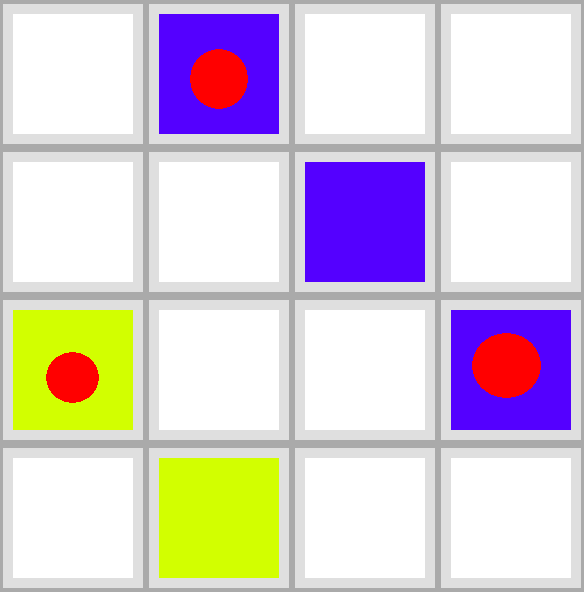
\includegraphics[width=0.3\textwidth]{dansgolf_sample1}
    \caption{Sýnidæmi 1}
    \label{fig:sample1}
\end{figure}
Eins og sjá má á Mynd~\ref{fig:sample1} þá þarf að kveikja á tveimur ljósum til að
lýsa upp alla dansara (sem eru táknaðir með rauðum deplum).

\section*{Stigagjöf}
Lausnin mun verða prófuð á miserfiðum inntaksgögnum, og er gögnunum skipt í
hópa eins og sýnt er í töflunni að neðan. Lausnin mun svo fá stig eftir því
hvaða hópar eru leystir.

\begin{tabular}{|l|l|l|l|}
\hline
Hópur & Stig & Inntaksstærð & Önnur skilyrði \\ \hline
1     & 25   & $1 \le N, M \leq 500$, $K \leq N\times M$ & $N = M$ \\ \hline
2     & 25   & $1 \le N, M \leq 500$, $K \leq N\times M$ &  \\ \hline
3     & 25   & $1 \le N, M \leq 10^9$, $K \leq 500$ & \\ \hline
4     & 25   & $1 \le N, M \leq 10^9$, $K \leq 2\cdot 10^5$ & \\ \hline
\end{tabular}

